% ============================================================================
% Cross-Model KV Transfer Needs Functional Compatibility
% Rewritten after the corrected-evaluation audit (paper/audit/METRIC_CORRECTION.md).
% Figures: paper/figures/gen_paper_figures.py (figures4papers house style).
% Every empirical number here is transcribed from the project result summaries
% named in the Reproducibility statement. Quantities that were not retained in
% those summaries are stated as such in the text; the \need{} macro is unused.
% ============================================================================
\documentclass[11pt]{article}

\usepackage[margin=1in]{geometry}
\usepackage[utf8]{inputenc}
\usepackage[T1]{fontenc}
\usepackage{booktabs}
\usepackage{graphicx}
\usepackage{multirow}
\usepackage{amsmath}
\usepackage{amssymb}
\usepackage[colorlinks=true,linkcolor=blue,citecolor=blue,urlcolor=blue]{hyperref}

\newcommand{\dll}{\Delta\text{LL}}
\newcommand{\emscore}{\text{EM}}
\newcommand{\need}[1]{\textbf{[NEEDS DATA: #1]}}
\setlength{\emergencystretch}{2.5em}
\setlength{\tabcolsep}{4pt}

% --- PDF metadata (arXiv submission) ---------------------------------------
% The author list must be the real one before posting; this draft is anonymous.
\hypersetup{
  pdftitle={Cross-Model KV Transfer Needs Functional Compatibility: Why Representation Alignment Is Not Enough},
  pdfauthor={Anonymous Author(s)},
  pdfsubject={Machine Learning; Natural Language Processing; Efficient Inference},
  pdfkeywords={KV cache transfer, cross-model inference, functional compatibility, representation alignment, evaluation methodology, parameter-efficient adaptation},
  bookmarksnumbered=true,
}

\title{Cross-Model KV Transfer Needs Functional Compatibility: \\
Why Representation Alignment Is Not Enough}

\author{Anonymous Author(s) \\ \texttt{anonymous@example.com}}
\date{}

\begin{document}
\maketitle

% ============================================================================
\begin{abstract}
Transferring key--value (KV) caches between language models promises to avoid
recomputation when a model is upgraded or an ensemble is assembled. We revisit
this claim within the Qwen3 family ($0.6$B--$8$B; six teacher--student pairs;
three seeds) and report a diagnostic negative result followed by a constructive
fix.

The evaluation protocol we used in earlier versions of this work overstates
transfer. Its greedy exact-match (EM) metric is computed on a cache that has
already been advanced through the query and the gold answer, and it re-feeds the
final query token as the first generation input; both defects are in that
implementation, and we validate the corrected evaluator against a full-prefill
reference on the whole Self test set (normalized-EM agreement
$0.929$--$0.982$; first-token top-1 agreement $0.929$--$0.982$; median $KL$
$0.001$--$0.005$ nats). The residual is a low-precision attention-kernel path
difference rather than a defect in cache construction or position handling: a
cache round-trip and an explicit position offset each reproduce the reference
bit for bit, and the same residual appears under eager attention. The validator
repeats on SQuAD (top-1 agreement $0.933$). Under that evaluator, no pair
averages more than $0.149$ EM for keys or
$0.065$ for the joint arm over three seeds (largest single seed $0.161$),
against
$0.44$--$0.90$ for the student's own cache; on the flagship $8$B$\to0.6$B pair
all three teacher arms are $0.000$, and V-only exceeds $0.15$ on one pair only
($8$B$\to4$B, $0.440$ against a Self of $0.815$). Teacher-forced
log-likelihood, which earlier work reports as transfer, is not a transfer
metric: over three seeds a wrong document ($+2.61$ vs $+2.62$), a
moment-matched random Gaussian key ($+2.33$), and an all-zero cache ($+2.75$)
reproduce $89$--$105\%$ of the K-only gain while each yields EM $\approx 0$,
against $0.899\pm0.010$ for the student's own cache. A control that breaks the
key--value correspondence instead of permuting both drives EM to $0.000$, so the
evaluator does detect content corruption. SQuAD replicates
the negative result (Self $0.367$; K-only, V-only, and Joint $0.000$; K-only
$\dll$ $+5.24$).

The failure lies in how the receiving model reads the state. Under a mapper fit
in representation space, layer alignment looks irrelevant: scrambling the layer
map costs nothing. Under a mapper fit in consumption space the same scrambling
collapses V-only EM from $0.91$ to $0.11$--$0.23$, so the earlier null result was
a floor effect of the mapper and alignment does matter once the consumer reads
the state correctly. Two failures are kept apart below: under mapped teacher keys
the student's top-1 attention agreement with its own routing is $0.59$--$0.70$
(a key-side diagnostic), while the value arm, which never sees a mapped key, is
limited by how the receiver consumes it. Fitting the value mapper where the
student reads value raises V-only EM from $0.113$ to $0.90$--$0.94$
($1.7$B$\to0.6$B) and from $0.000$ to $0.25$--$0.27$ ($8$B$\to0.6$B), while a
shuffled-target mapper stays at $0.08/0.07$. Raw representation error does not
rank these variants (rank correlation $-0.10$ pooled over five variants and six
runs, per-run range $[-0.60,-0.10]$), whereas error measured after the
student's attention output and after its $o$-projection does ($-1.00$ and
$-0.80$, range $[-1.00,-0.80]$ in every run). A rank-8 correction of the
student's output projections ($\sim$$0.7$M parameters), trained by next-token
cross-entropy on calibration answers under injected teacher KV, restores
K/V/Joint EM to $0.94/0.94/0.83$
($1.7$B$\to0.6$B; Joint spread $0.55$--$0.96$ across seeds) and
$0.79/0.36/0.47$ ($8$B$\to0.6$B), measured against an adapted Self of $0.940$ on
the flagship pair rather than the unadapted $0.899$. Holding the final adapter
fixed and destroying the injected content drops EM to the floor on
$1.7$B$\to0.6$B, where correct teacher KV answers $0.905\pm0.083$ of questions
against at most $0.179$ for wrong-document, random, and zero caches (three
seeds); on $8$B$\to0.6$B the same margin is $+0.071$ on average, which our
pre-registered gate does not let us separate from no margin, and we report it as
unresolved. The same adapter trained on student states stays much lower
($0.20/0.35/0.18$ and $0.11/0.11/0.12$), and one trained on shuffled-document
teacher states is intermediate (Joint $0.46$ and $0.13$). The repair does not
transfer across domains, and on SQuAD it does not reappear within one either:
retrained on SQuAD calibration documents, every transfer arm still answers
$0.000$ of the held-out questions across three document splits, so what the
synthetic domain repairs is bound to that task distribution; we name this
\emph{task-conditioned} functional compatibility. All experiments are
within a single model family, and the
adapter is trained on the task distribution it is evaluated on.
\end{abstract}
% ============================================================================
\section{Introduction}

Prefilling a long document is expensive, and the resulting KV cache is discarded
whenever a model is upgraded, a smaller model is substituted for a larger one, or
an ensemble is assembled. Reusing that state across models would remove the
recomputation. Recent work maps caches between models with closed-form or learned
linear translators~\cite{heo2026crossmodel,fu2026c2c,lee2026translators,dery2026latentalign}
and reports that keys can be predicted much more accurately than values. The
natural reading is that addressing geometry is shared within a model family while
content is bound to the weights that produced it, so keys transfer and values do
not.

This paper argues that this reading rests on two measurement choices that do not
survive scrutiny, and that once they are corrected the question changes from
\emph{which component transfers} to \emph{when a consumer can read a transferred
state}. The first choice is the evaluator: in the path we used in earlier versions
of this work, the greedy exact-match (EM) metric is computed on a cache that has
already been advanced through the query and the gold answer, and the final query
token is re-fed as the first generation input. Both defects are in that
implementation; we did not audit third-party implementations. The second
choice is the primary metric itself: teacher-forced answer log-likelihood, which
is treated as evidence of transfer.

We study six teacher--student pairs within the Qwen3 family
($0.6$B--$8$B; three seeds; $n=56$ held-out questions per seed;
Figure~\ref{fig:setting}). Our contributions are:

\begin{enumerate}
\item \textbf{An evaluation principle.} Teacher-forced answer likelihood is not
  evidence that a state was functionally transferred. Over three seeds a
  wrong-document cache ($+2.61$ vs $+2.62$), a moment-matched random Gaussian
  key ($+2.33$), and an all-zero cache ($+2.75$) reproduce $89$--$105\%$ of the
  K-only likelihood gain while each yields EM $\approx 0$, against
  $0.899\pm0.010$ for the student's own cache, and the evaluator is not
  insensitive to content: shuffling one side of the student's own cache while
  leaving the other in place drives EM to $0.000$ in every seed and both pairs,
  whereas the \emph{same} permutation applied to both sides leaves it at
  $0.86$--$0.93$ and therefore tests nothing. This claim holds independently of
  any implementation. Separately, the greedy-EM path we used in earlier versions
  of this work contained two defects that inflated our own measurements; we fix
  both, require generation to start from a fresh cache, and validate the
  corrected evaluator against a full-prefill reference on the complete
  $56$-item Self test set of every student size under study ($0.6$B, $1.7$B,
  $4$B; normalized-EM agreement $0.929$--$0.982$, first-token top-1 agreement
  $0.929$--$0.982$, median $KL$ $0.001$--$0.005$ nats). A cache round-trip and
  an explicit position offset each reproduce the reference bit for bit while the
  same residual persists under eager attention, so the residual is a
  low-precision attention-kernel path difference rather than a defective
  evaluator. Under it, no pair's three-seed mean exceeds $0.149$ EM for keys and
  $0.065$ for the joint arm, against $0.44$--$0.90$ for the student's own cache,
  and the negative result replicates on SQuAD (Self $0.367$; K-only, V-only, and
  joint $0.000$), where the same validator holds (top-1 agreement $0.933$). Our
  own pre-registered gate for this project used the same EM metric; we withdraw
  its task-metric clause, while its likelihood clause stands.

\item \textbf{A functional compatibility decomposition.} A handed-off cache
  perturbs the student's output through two terms, a routing term
  $(\hat A-A_S)V_SW_O^S$ and a consumption term $\hat A(\hat V-V_S)W_O^S$, and
  the four arms switch them on and off (Section~\ref{sec:decomp}). We use the
  identity as the frame that names the two compatibility requirements, not as a
  claim that task performance decomposes additively, and we identify the terms
  by intervention. The key arm moves the receiver's routing: top-1 attention
  agreement with its own routing is $0.70$ ($1.7$B$\to0.6$B) and $0.59$
  ($8$B$\to0.6$B), with routing total-variation $0.167$ and $0.251$. The value
  arm never sees a mapped key, so its failure is not addressing; it is a
  consumption-space mismatch, which is why the two failures are kept apart
  rather than folded into one mechanism.

\item \textbf{Consumer-space alignment.} The target of alignment matters more
  than its accuracy. Fitting the value mapper where the student reads value
  recovers most of V-only transfer without touching a single consumer weight:
  an attention-output-aware mapper raises EM from $0.113$ to $0.935$
  ($1.7$B$\to0.6$B) and from $0.000$ to $0.250$ ($8$B$\to0.6$B), a
  $W_O$-aware mapper reaches $0.899$ and $0.268$, and a mapper with shuffled
  targets stays at $0.077$ and $0.065$. Measuring the same five mapper variants
  against the state they produce separates the two spaces: pooled over six runs,
  raw representation error does not rank them (rank correlation $-0.10$ against
  EM), while attention-output error and $o$-projection-space error do ($-1.00$
  and $-0.80$), with the shuffled-target control the visible exception. Layer
  alignment is masked rather than absent: with a representation-space mapper the
  value arm sits at the floor (corrected V-only EM $\le0.143$ in every seed) and
  offsetting or permuting the layer map changes almost nothing, whereas with the
  consumption-space mapper the same scrambling costs most of the transfer,
  V-only EM falling from $0.911$ to $0.107$--$0.232$ with non-overlapping
  document-clustered intervals.

\item \textbf{Repairability and its boundary.} A rank-8 correction of the
  student's output projections ($\approx0.7$M parameters), trained by next-token
  cross-entropy on calibration answers under injected teacher KV while the
  student and mapper stay frozen, restores K/V/joint EM to $0.94/0.94/0.83$ for
  $1.7$B$\to0.6$B (joint arm spread $0.55$--$0.96$ across seeds) and
  $0.79/0.36/0.47$ for $8$B$\to0.6$B, measured against an \emph{adapted} Self of
  $0.940\pm0.041$ rather than the unadapted $0.899$. With the \emph{final}
  $20$-epoch adapter frozen and the injected content destroyed, the arms
  separate cleanly on $1.7$B$\to0.6$B (correct teacher KV $0.905\pm0.083$ across
  three seeds, against at most $0.179$ for wrong-document, random, and zero
  caches) but not on $8$B$\to0.6$B, where the mean margin $+0.071$ falls below
  the $0.10$ our pre-registered gate requires and one seed's clustered interval
  includes zero; we report that as unresolved rather than lowering the bar. The
  same adapter trained on the student's own states stays far lower
  ($0.20/0.35/0.18$ and $0.11/0.11/0.12$), so the recovery requires the
  teacher-state distribution rather than a generic correction of the consumer.
  The repair is also bounded by the task distribution. On SQuAD it does not appear
  out of domain, and it does not reappear within the domain either: retraining
  the mapper and the adapter on SQuAD calibration documents still answers
  $0.000$ of the held-out questions on every transfer arm across three document
  splits, even though the same recipe recovers $0.94$ V-only EM on the synthetic
  distribution. Compatibility is therefore conditioned on the task distribution
  and not a property of the model pair alone.

\end{enumerate}

The practical message separates two levels of compatibility. At the level of
\emph{state space}, matching raw KV representations is not sufficient: a mapper
that minimises representation error can leave the state unusable. At the level of
\emph{consumption space}, alignment is what matters, and it can be restored in two
ways---by fitting the mapper where the student actually reads value, and, when that
is not enough, by a small adaptation of the consumer itself. The second level is
where our evidence is clearest: on the equal-depth pair the consumption-space
value mapper recovers the value arm without changing a single consumer weight and
only the residual gap needs the adapter, whereas on the flagship pair the mapper
alone recovers about a quarter of Self and the adapter is required. The
key-side mismatch is diagnosable (routing divergence) and the value-side one is
repairable; the general lesson is that representation alignment is the wrong
target object, because the quantity that decides usability is the error the
receiver makes on the state it is handed, measured where it consumes it.
Evaluations of cross-model transfer should therefore report task performance
under a corrected evaluator and include content controls.

\begin{figure}[t]
\centering
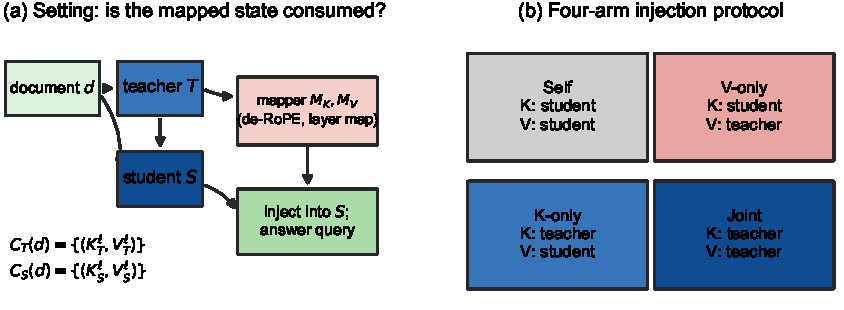
\includegraphics[width=\textwidth]{figures/fig_setting.pdf}
\caption{Setting and protocol. (a) A document is prefilled by a teacher and by a
student; a mapper aligns teacher state to student space (keys are de-RoPE'd
before mapping). We ask whether the mapped state is \emph{consumed}, not merely
whether it is linearly predictable. (b) The four-arm protocol. Self is the
student's own cache and serves as the reference; K-only and V-only isolate
addressing and content; Joint is the full handoff.}
\label{fig:setting}
\end{figure}
% ============================================================================
\section{Related Work}

\subsection{Cross-Model KV Cache Transfer}
\label{sec:rw-transfer}
The closest line of work maps KV state across models.
Heo et al.~\cite{heo2026crossmodel} introduce a closed-form per-head ridge mapper
with RoPE-stripped keys and cross-layer source selection for prefill reuse within
a model family, and report that keys are more predictable than values.
Cache-to-Cache~\cite{fu2026c2c} transfers semantic states between LLMs for direct
communication; Mixture-of-Translators~\cite{lee2026translators} translates caches
across heterogeneous LLMs; LatentAlign~\cite{dery2026latentalign} aligns latent
spaces through KV-cache alignment. Prior work transfers full KV states with
engineered mappings and evaluates with teacher-forced likelihood or greedy
overlap. Our contribution is diagnostic and constructive: our legacy task
evaluator could report apparent transfer where none exists functionally, and,
more generally, teacher-forced likelihood alone is insufficient evidence of
functional transfer. We localize the failure to the consumer and recover transfer
by adapting the consumer rather than the state.

\subsection{KV Cache Optimization}
\label{sec:rw-kvopt}
FlashAttention~\cite{dao2022flashattention} reduces memory traffic; speculative
decoding~\cite{leviathan2023fast,chen2023accelerating} reduces latency; KV
quantization (KIVI~\cite{kivi2024icml}, KVQuant~\cite{kvquant2024nips})
compresses the cache. These operate within one model; we study cross-model
consumption of the state itself.

\subsection{Compression, Distillation, Merging, and Stitching}
\label{sec:rw-merge}
Quantization~\cite{frantar2023gptq,dettmers2024qlora}, distillation
\cite{hinton2015distilling,touvron2023llama}, model
merging~\cite{ties2023merging,dare2024icml}, and model
stitching~\cite{bansal2021stitching} modify or combine weights. Our consumption
adapter is closest in spirit to parameter-efficient adaptation: it adds a small
low-rank module while the pretrained model and the state mapper stay frozen.

\subsection{Attention and Positional Structure}
\label{sec:rw-attn}
The Transformer~\cite{vaswani2017attention} separates keys (addressing) from
values (content); RoPE~\cite{su2024rope} adds positional structure to keys. We
strip positional structure before mapping keys, and treat the consumer's routing
($A=\mathrm{softmax}(QK^{\top})$) and output pathway ($O=AVW_O$) as the objects
of study.

% ============================================================================
\section{Method}

\subsection{Problem setup}
\label{sec:problem-setup}
We are given a teacher $T$ and a student $S$ with $L_T$ and $L_S$ layers. For a
document $d$, each model produces a KV cache
$C_m(d)=\{(K_m^\ell,V_m^\ell)\}_{\ell=1}^{L_m}$. A mapper maps teacher state into
student space using a layer map $\pi:[L_S]\to[L_T]$ (proportional for unequal
depth, identity for equal depth). Keys are de-RoPE'd before mapping and the
student's positions are re-applied afterwards. The mapped document state is
injected into the student, which sees only the query at generation time; we then
measure whether it answers a held-out question.

\subsection{Injection protocol}
\label{sec:injection}
Each evaluation sample yields four arms built from the document state
(Figure~\ref{fig:setting}b):
\textbf{Self} (student K and V), \textbf{K-only} (mapped teacher K with student
V), \textbf{V-only} (student K with mapped teacher V), and \textbf{Joint}
(mapped teacher K and V). Self is the reference: it measures the student's
ceiling when it reads its own state. K-only and V-only isolate addressing from
content; Joint is the full handoff.

\subsection{Functional compatibility decomposition}
\label{sec:decomp}
Let $O_S=A_SV_SW_O^S$ be the student's attention output when it reads its own
cache, and $\hat O=\hat A\hat VW_O^S$ its output when it reads a handed-off
cache, with the student's output projection $W_O^S$ frozen. The perturbation
splits exactly,
\begin{equation}
\hat O-O_S
= \underbrace{(\hat A-A_S)V_SW_O^S}_{\text{routing term}}
+ \underbrace{\hat A(\hat V-V_S)W_O^S}_{\text{consumption term}} .
\label{eq:decomp}
\end{equation}
The four arms of Section~\ref{sec:injection} switch the two terms on and off.
K-only sets $\hat V=V_S$ and leaves the routing term alone; V-only sets
$\hat A=A_S$ and leaves the consumption term alone; Joint carries both, together
with their interaction. Equation~\eqref{eq:decomp} is an identity about the
perturbation, not a claim that task performance decomposes additively: exact
match is a discrete function of the output, and the likelihood-scale interaction
changes sign across pairs (Appendix~\ref{app:factorial}). We use it as the frame
that names two compatibility requirements---the receiver's routing has to
accommodate handed-off keys, and its consumption pathway has to accept handed-off
values---and we test each requirement by intervention rather than by arithmetic.
The identity says which term is switched on in each arm; it does not say which
term limits task performance, because the two terms are measured on a scale
(the output perturbation) that is not the task metric.

\subsection{Corrected evaluation}
\label{sec:eval-protocol}
The implementation used in earlier versions of this work advances a single cache
through the query \emph{and the gold answer} during scoring, then calls greedy
generation on that same mutated cache, so the model reproduces an answer it has
just been shown. A second defect re-feeds the final query token as the first
generation input, which degrades to punctuation loops once the cache is
perturbed. Both defects are in that implementation, which we audited; we did not
audit third-party implementations. We use a corrected evaluator in which
teacher-forced log-likelihood and greedy generation each start from a
\emph{fresh} cache and the first generated token is taken from the prefill
logits. We validate the corrected evaluator against a full-prefill reference
implementation on the complete $56$-item Self test set of three student sizes
(Figure~\ref{fig:evalcheck}). Normalized answer exact match agrees on $0.964$
($0.6$B), $0.929$ ($1.7$B), and $0.982$ ($4$B) of the items and differs by at
most two items per student; first-token top-1 agreement is $0.929$, $0.929$, and
$0.982$; and the median $KL$ between the two first-token distributions is
$0.0047$, $0.0015$, and $0.0010$ nats. Token-level greedy agreement is lower
($0.786$, $0.804$, $0.929$) because greedy tokenization drifts without changing
the extracted answer, and the largest absolute logit error is $1.344$, $0.875$,
and $0.969$. We attribute that residual rather than only reporting it. Repeating
the document prefill is deterministic (bit-identical caches), and the injected
path reproduces the reference bit for bit both when the captured cache is
installed directly instead of through a numpy round-trip and when the query's
position offset is passed explicitly. What remains is the attention kernel path
itself---a one-token query against a cache versus a full-sequence prefill---which
accounts for the entire residual (on an eight-item probe, the largest absolute
logit error is $0.844$ and the median $KL$ is $0.005$ nats) and does not shrink
under eager attention. The disagreements are near-ties resolved differently at bf16
precision, not a defect in how the cache or the positions are handled. The same
validator holds on the second domain (Section~\ref{sec:second-domain}).

\begin{figure}[t]
\centering
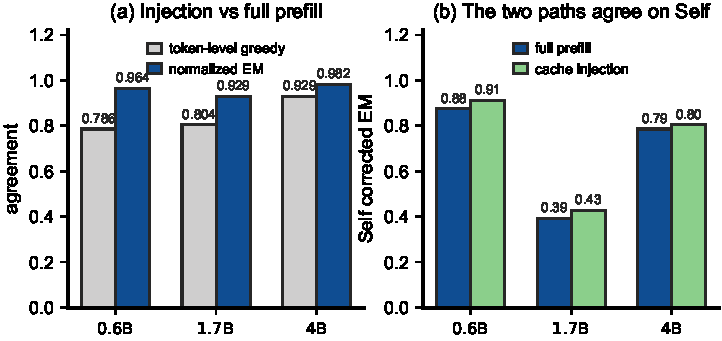
\includegraphics[width=0.86\textwidth]{figures/fig_evalcheck.pdf}
\caption{Validator for the corrected evaluator: cache injection against a
full-prefill reference on the complete $56$-item Self test set of each student
size, seed 0. (a) Agreement between the two paths. Token-level greedy agreement
is lower than normalized exact-match agreement because greedy tokenization drifts
without changing the extracted answer. (b) First generated token's logits agree
to within $1.344$ in absolute value, first-token top-1 agreement is
$0.93$--$0.98$, and Self exact match under the two paths differs by at most two
items. An attribution probe places the whole residual on the attention kernel
path: repeated capture, the cache round-trip, and an explicit position offset are
each exact.}
\label{fig:evalcheck}
\end{figure}

Throughout, \emph{corrected EM} denotes greedy exact match under this evaluator.
All EM numbers reported in the previous version of this work were produced by the
defective path and are withdrawn; the correction note and the legacy tables are
provided as supplementary material.

\subsection{Mappers}
\label{sec:mappers}
The default mapper is a per-(layer, head) affine ridge map fit on calibration
data. We additionally define two consumer-space mappers for values:
(i) an \textbf{attention-output-aware} mapper that matches $A_S V_T \to A_S V_S$
on calibration, i.e.\ it is fit where the student reads value; and (ii) a
\textbf{$W_O$-aware} mapper that additionally projects through the student's
output projection and, per KV head $h$, satisfies
$M_h W_{O,q} \approx N_q$ for every grouped query head $q$ in the GQA group,
where $N_q$ is the ridge map $A_q V_{T,h} \to A_q V_{S,h} W_{O,q}$. A
shuffled-target mapper, fit to the same objective with targets taken from a
\emph{different} document, is the content-specificity control. All mappers are
trained on the calibration split only.

\subsection{Consumption adapter}
\label{sec:adapter}
To test whether the receiving model can be made compatible, we add a rank-$r$
low-rank correction to the student's attention projections,
$\mathrm{proj}'(x)=Wx+B(Ax)$ with $B$ initialized to zero, and train only
$\{A,B\}$ by next-token cross-entropy on the calibration split with mapped
teacher KV injected; the student and the mapper are frozen. Unless stated
otherwise $r=8$, the adapted module is \texttt{o\_proj}, the optimizer is Adam
with learning rate $10^{-3}$ for $20$ epochs, and gradients are clipped at $1.0$.
We ablate which projection is adapted and which states the adapter is trained on
(teacher, student, or shuffled-document teacher KV). Each training condition
trains its own adapter from scratch, and that single adapter is then evaluated on
all four injection arms; parameters are not shared across conditions.
% ============================================================================
\section{Experimental Setup}

\subsection{Models and pairs}
\label{sec:models}
All models are from the Qwen3 family: $0.6$B, $1.7$B, $4$B, and $8$B
parameters. The $8$B and $4$B models have $36$ layers and the $1.7$B and $0.6$B
models have $28$ layers; all use $8$ key/value heads and head dimension $128$,
with grouped-query attention at the query side. We evaluate all six ordered pairs
in which the teacher is strictly larger than the student: $8$B$\to0.6$B,
$4$B$\to1.7$B, $4$B$\to0.6$B, $8$B$\to1.7$B, $1.7$B$\to0.6$B, and
$8$B$\to4$B. Two pairs are equal-depth ($8$B$\to4$B, $1.7$B$\to0.6$B) and four
are unequal-depth.

\subsection{Data}
\label{sec:data}
We use a synthetic out-of-domain (OOD) corpus: a hidden knowledge graph of
fictional entities is rendered into project-status documents, questions are
sampled with hop depths $1$--$4$, and answers are verified programmatically.
Splits are made by entity cluster (train $70$ / validation $28$ / test $56$
questions per seed), so test entities never appear in training. Test questions
come from $8$ unique documents (about seven questions per document), so we report
document-clustered bootstrap intervals for the control suite and interpret
per-sample intervals with this clustering in mind. As a second domain we evaluate
on SQuAD ($n=30$ held-out questions) with a mapper calibrated only on the
synthetic OOD training split.

\subsection{Metrics and controls}
\label{sec:metrics}
Our primary task metric is corrected greedy exact match. Teacher-forced answer
log-likelihood (LL), relative to the Self arm of the same sample, is reported as
a secondary and explicitly non-task quantity. Content controls are a
wrong-document cache (a different project's state), a random Gaussian key with
matched per-layer moments, a random KV pair, an all-zero cache, an identity
(unmapped) V-only injection, and two \emph{correspondence-breaking} shuffles of
the student's own cache: one permutes the key token order and leaves values in
place, the other is its mirror on values. We also compute a same-permutation arm
that reorders keys and values together; we report it only as an invariance check,
because attention is invariant to a shared reordering of $K$ and $V$ and such an
arm cannot detect content corruption. Every other control destroys content. The
shuffles act on the student's own state, so both are pair-independent by
construction, and their agreement across pairs is a consistency check rather than
an independent result. For the adapter we additionally train on student KV and on
shuffled-document teacher KV.

\subsection{Statistical protocol}
\label{sec:stats-protocol}
Every comparison in this paper is run with three seeds (0, 1, 2), each with its
own entity-cluster split. We report mean $\pm$ standard deviation across seeds
for all main quantities. Significance of arm differences is assessed with paired
Wilcoxon signed-rank tests against Self on the same samples, with
document-clustered bootstrap CI95 where a per-sample interval is reported. We
report $p$ values only where the corresponding report gives them, and we name the
seed or seed aggregate for each.

\subsection{Confirmatory and exploratory analyses}
\label{sec:analyses}
We separate these explicitly, because the metric correction changed the status of
part of our own earlier work.

\emph{Confirmatory.} The four-arm injection protocol, the six pairs, the
three-seed requirement, and the pre-registered G0 gate predate this revision. The
content-control suite, the layer-map ablation, the held-out layer scan, the
routing/mapper comparison, the evaluator validator, the repaired-regime layer
scrambling, the adapter causality test, and the cross-domain repair attempt were
all specified in a written revision plan, with a decision rule, before the
corresponding runs; the plan and the raw reports are in the repository.

\emph{Exploratory.} The corrected evaluator, the consumption adapter, the
projection ablation, the decomposition of the likelihood gains into K and V main
effects and their interaction (Appendix~\ref{app:factorial}), and the observation
that only equal-depth pairs show non-zero V-only EM were introduced after we
found the evaluator defects.
They are hypothesis-generating. Two of our earlier conclusions also moved:
scrambling the layer map, which we had reported as harmless, is harmful once the
mapper is fixed (Section~\ref{sec:layer-align}), and the flagship pair's adapter behaviour is
weaker than the equal-depth pair's.

\emph{Withdrawn.} Our pre-registered G0 gate was defined on the defective EM
metric, on the earlier calibration/evaluation split ($42$/$14$), where V-only
sat $+1.75$ above Self in answer likelihood ($-9.97 \pm 2.60$ against
$-11.72 \pm 2.07$, 95\% intervals overlapping). Its task-metric clause is
therefore withdrawn. We re-ran its likelihood clause after fixing a baseline
double-counting bug, on the current split ($70$/$56$), where V-only is at or
below Self in every seed ($\dll = -0.045$, $-0.219$, $-0.415$; $p = 0.024$,
$0.125$, $0.144$, none significant). The clause's verdict---V-only does not
transfer---is unchanged, and it rests on a re-run of the pre-registered test
rather than on the original run; it can no longer be read as a statement about
task performance.
% ============================================================================
\section{Results}

\subsection{Teacher states do not answer questions}
\label{sec:teacher-states}
Table~\ref{tab:main} and Figure~\ref{fig:fourarm} report corrected EM and LL for
all six pairs over three seeds. The LL deltas reproduce the published values
exactly (e.g.\ $8$B$\to0.6$B K-only $+2.62$, V-only $-0.23$), which confirms that
the pipeline itself is unchanged and that only the EM path was broken.

The student answers most questions from its own cache ($0.899 \pm 0.010$ for the
three pairs with a $0.6$B student, $0.440 \pm 0.010$ for the two with a $1.7$B
student, $0.815 \pm 0.021$ for the $4$B student). No teacher arm comes close.
Averaged over seeds, K-only is at most $0.149 \pm 0.010$ ($8$B$\to4$B) and Joint
at most $0.065 \pm 0.055$ ($8$B$\to4$B); the largest value any single seed
reaches on either arm is $0.161$ (K-only) and $0.125$ (Joint), both on
$8$B$\to4$B. On the flagship $8$B$\to0.6$B pair all three
teacher arms are $0.000$ in every seed. The single arm above $0.15$ is V-only on
$8$B$\to4$B, at $0.440 \pm 0.010$---a little over half of that pair's Self
($0.815$)---and V-only is $0.000$ on all four unequal-depth pairs. No other
teacher arm exceeds $0.15$ when averaged over seeds. With documents as the
resampling unit (eight clusters per seed), that pair's V-only arm carries CI95
$[0.375, 0.482]$, $[0.429, 0.482]$, and $[0.429, 0.482]$ over the three seeds:
every interval excludes zero and every one sits far below the same seed's Self
($0.804$--$0.839$). The same resampling leaves K-only within $[0.071, 0.250]$
and Joint at or below $0.179$, so clustering widens the intervals without
changing any arm ordering.

Meanwhile the same injections raise teacher-forced likelihood substantially:
K-only by up to $+8.52$ ($8$B$\to4$B) and Joint by up to $+8.37$, with the
flagship at $+2.62$ and $+4.52$. Figure~\ref{fig:fourarm} shows the dissociation
directly: the arms that move likelihood most are not the arms that answer
questions.

\begin{table}[t]
\centering
\small
\caption{Corrected four-arm scan, six pairs, three seeds, $n=56$.
EM is corrected greedy exact match; $\dll$ is teacher-forced answer
log-likelihood relative to Self. Values are mean $\pm$ std over seeds.
A blank std means the source reports no dispersion for that cell; every such
cell is a $0.000$ arm in all three seeds. Document-clustered CI95 for EM
(clusters $=$ documents, eight per seed) is computed for every seed from the
archived per-sample rows and is quoted in the text for the arms on which a claim
depends.}
\label{tab:main}
\begin{tabular}{lcccccccc}
\toprule
 & & \multicolumn{4}{c}{Corrected EM} & \multicolumn{3}{c}{$\dll$ vs Self} \\
\cmidrule(lr){3-6}\cmidrule(lr){7-9}
Pair & Self & K & V & J & K & V & J \\
\midrule
$8$B$\to0.6$B   & $0.899{\pm}0.010$ & $0.000$ & $0.000$ & $0.000$ & $+2.62{\pm}0.29$ & $-0.23{\pm}0.19$ & $+4.52{\pm}0.15$ \\
$4$B$\to1.7$B   & $0.440{\pm}0.010$ & $0.054{\pm}0.018$ & $0.000$ & $0.024{\pm}0.010$ & $+2.90{\pm}0.09$ & $+2.91{\pm}0.21$ & $+2.31{\pm}0.25$ \\
$4$B$\to0.6$B   & $0.899{\pm}0.010$ & $0.000$ & $0.000$ & $0.006{\pm}0.010$ & $+1.58{\pm}0.02$ & $-1.22{\pm}0.05$ & $+2.50{\pm}0.52$ \\
$8$B$\to1.7$B   & $0.440{\pm}0.010$ & $0.000$ & $0.000$ & $0.012{\pm}0.021$ & $+1.04{\pm}1.53$ & $+5.63{\pm}0.04$ & $+4.69{\pm}0.27$ \\
$1.7$B$\to0.6$B & $0.899{\pm}0.010$ & $0.030{\pm}0.010$ & $0.113{\pm}0.052$ & $0.000$ & $-0.82{\pm}0.02$ & $+0.63{\pm}0.17$ & $-2.25{\pm}0.14$ \\
$8$B$\to4$B     & $0.815{\pm}0.021$ & $0.149{\pm}0.010$ & $0.440{\pm}0.010$ & $0.065{\pm}0.055$ & $+8.52{\pm}0.28$ & $+2.52{\pm}0.07$ & $+8.37{\pm}0.28$ \\
\bottomrule
\end{tabular}
\end{table}

\begin{figure}[t]
\centering
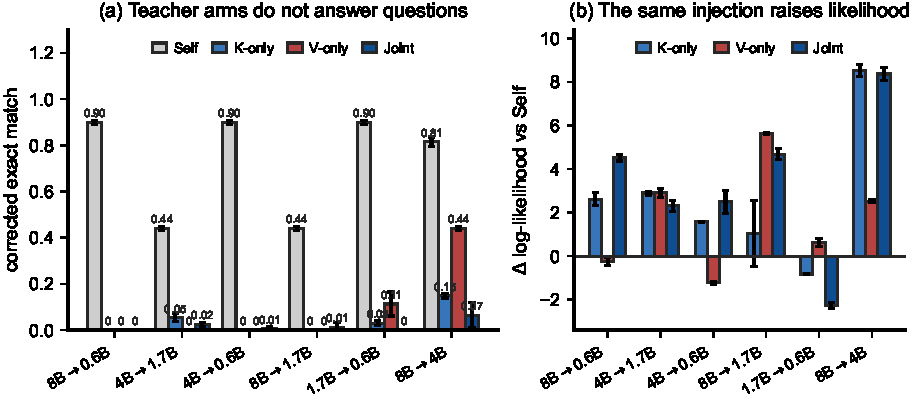
\includegraphics[width=\textwidth]{figures/fig_fourarm.pdf}
\caption{Corrected four-arm scan (three seeds). (a) Only the student's own cache
answers questions. Unlabelled bars are $0.00$. (b) The same injections raise
teacher-forced likelihood, most strongly where no answers are produced. Error
bars are std over seeds where the source reports it.}
\label{fig:fourarm}
\end{figure}
\subsection{Log-likelihood gains are content-agnostic}
\label{sec:controls}
The likelihood gains that a likelihood-only protocol would read as transfer do
not carry document content (Table~\ref{tab:controls},
Figure~\ref{fig:controls}). Over three seeds, a wrong-document cache---a different
project's state---leaves the K-only likelihood gain essentially unchanged
($+2.61 \pm 0.31$ vs $+2.62 \pm 0.29$); a random Gaussian key with matched
per-layer moments recovers $89\%$ ($+2.33 \pm 0.27$); an all-zero cache recovers
$105\%$ ($+2.75 \pm 0.01$), exceeding the real K-only injection; and the joint
arm behaves the same way ($+4.50$ wrong-document vs $+4.52$ real). At seed 0,
where the source reports document-clustered intervals, the K-only gain has CI95
$[+2.21, +2.64]$ and the zero-KV gain $[+2.49, +3.00]$, so the control intervals
overlap the real arm's.

Every one of these arms yields corrected EM at or near $0$. A control that does
break the correspondence is informative: permuting the token order of the
student's own keys while leaving its values aligned to their positions drives EM
to $0.000$ in all three seeds, and the mirror control on values does the same
(Table~\ref{tab:controls}). The same-permutation arm that the previous draft
relied on is not a content control---attention is invariant to a shared
reordering of $K$ and $V$---and it returns $0.929$, $0.875$, and $0.857$ across
seeds, which is what that invariance predicts; we report it only as a check that
the evaluator is not suppressing a permutation-invariant quantity.

The evaluator is therefore not insensitive to context: it scores
$0.899 \pm 0.010$ on the student's own cache, returns nothing for
teacher-injected states, and returns nothing when the key--value correspondence
is destroyed. The same pattern holds over three seeds for the equal-depth pair
$1.7$B$\to0.6$B. There the real K-only injection \emph{lowers} answer
log-likelihood ($-0.82 \pm 0.02$) and answers $0.030 \pm 0.010$ of questions,
while content-free caches raise it (zero KV $+2.75 \pm 0.01$, random K
$+2.33 \pm 0.27$, wrong-document K $-0.78 \pm 0.06$) and answer at most $0.036$;
a wrong-document cache is indistinguishable from the real one on both axes. Here
the dissociation runs the other way---likelihood improves as content is
destroyed---which is the same failure of the likelihood metric seen from the
opposite side. Unlike at $8$B, however, the content-free arms do not exceed the
real arm on every comparison, and the content-free arms are pair-independent by
construction, so we read the $1.7$B suite as corroborating the $8$B controls
rather than as an independent replication.

\begin{table}[t]
\centering
\small
\caption{Content controls on $8$B$\to0.6$B, corrected evaluator, three seeds
(mean $\pm$ std). ``Share'' is the arm's $\dll$ divided by the
K-only $\dll$ of the same runs. The last three rows act on the student's own
cache rather than on the teacher state, so they are identical on every pair by
construction; the first five are teacher- or content-free arms.}
\label{tab:controls}
\begin{tabular}{lccc}
\toprule
Arm & $\dll$ vs Self & Corrected EM & Share of K-only gain \\
\midrule
K-only (real)          & $+2.62{\pm}0.29$ & $0.000$ & $100\%$ \\
Wrong-document K       & $+2.61{\pm}0.31$ & $0.000$ & $100\%$ \\
Random Gaussian K      & $+2.33{\pm}0.27$ & $0.012{\pm}0.010$ & $89\%$ \\
Zero KV                & $+2.75{\pm}0.01$ & $0.000$ & $105\%$ \\
Joint (real)           & $+4.52{\pm}0.15$ & $0.000$ & --- \\
Wrong-document Joint   & $+4.50{\pm}0.18$ & $0.000$ & --- \\
\midrule
Shuffled K (student)   & $-1.19{\pm}0.10$ & $0.000$ & --- \\
Shuffled V (student)   & $-1.28{\pm}0.04$ & $0.000$ & --- \\
Same permutation, K and V (student) & $-0.01{\pm}0.00$ & $0.887{\pm}0.037$ & --- \\
\bottomrule
\end{tabular}
\end{table}

\begin{figure}[t]
\centering
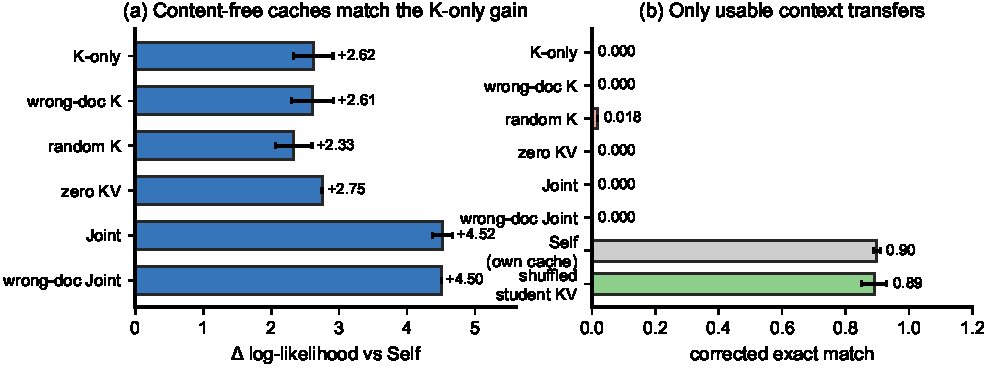
\includegraphics[width=\textwidth]{figures/fig_controls.pdf}
\caption{Content controls on $8$B$\to0.6$B. (a) The K-only and Joint likelihood
gains are matched or exceeded by wrong-document, random, and all-zero caches.
(b) None of the teacher or content-free arms answers questions, while the
student's own cache scores $0.899$. The evaluator reads usable context and
returns nothing for injected states. Error bars are std over seeds where
reported.}
\label{fig:controls}
\end{figure}

\subsection{Second domain}
\label{sec:second-domain}
On SQuAD, with a mapper calibrated only on the synthetic OOD split and $n=30$
held-out questions, corrected EM is $0.367$ for Self and $0.000$ for K-only,
V-only, and Joint in all three seeds. The validator repeats here unmodified: on
these $30$ Self items normalized-EM agreement is $0.933$, first-token top-1
agreement is $0.933$, and the median $KL$ is $0.005$ nats, with identical Self
exact match under both paths. The K-only likelihood gain is $+5.24$
averaged over three seeds ($+5.223$ at seed 0, Wilcoxon $p = 2.8\times10^{-6}$
against Self at that seed; V-only $+1.053$, $p=0.205$; Joint $+3.497$,
$p=1.9\times10^{-4}$). The K-only gain is significant at every seed
($p = 2.8\times10^{-6}$, $4.7\times10^{-7}$, $2.1\times10^{-7}$ for seeds
$0$--$2$); we report those per-seed tests instead of a pooled $p$, because the
per-example deltas a pooled test would need were not retained. The negative
result and the LL/EM dissociation therefore replicate out of domain, on data the
mapper never saw. Neither repair transfers to this set: the synthetic-trained
mapper and the synthetic-trained adapter both leave K-only and joint EM at
$0.000$ here (Section~\ref{sec:adapter-results},
Table~\ref{tab:squadrepair}). We note that the
legacy evaluator scored K-only at $0.733$ EM on this set while the corrected
evaluator scores it at $0.000$, and that the legacy Self score was $0.767$
against a corrected Self of $0.367$: the defect moved the reference point as well
as the arm. Whether this domain also fails when the repair is refit inside it is
the question Section~\ref{sec:adapter-results} answers, and it is what makes
compatibility task-conditioned rather than a property of the model pair.
% ============================================================================
\section{Analysis}

\subsection{Layer alignment matters once the consumer reads the state}
\label{sec:layer-align}
For the equal-depth pair $1.7$B$\to0.6$B we vary only the layer map and hold the
capability gap fixed (Figure~\ref{fig:layers}a). Under the affine mapper that
earlier work uses, the value arm is pinned at the floor and the layer map looks
irrelevant: proportional (identity) mapping gives corrected V-only EM
$0.05$--$0.14$ across three seeds, offsets of $\pm3$ and a random permutation
give $0.000$ in every seed, and the permutation even \emph{raises} the V
likelihood delta ($+1.35$ vs $+0.83$ at seed 0). We previously read this as layer
alignment being unimportant. It is a floor effect of the mapper: with the value
arm already at $0$, no layer map can make it worse.

Repeating the ablation with the consumption-space mapper of
Table~\ref{tab:mappers}, which lifts proportional V-only EM to $0.911/0.929/0.964$
across the three seeds (mean $0.935$), changes the answer. At seed 0 the same
offsets and permutation now cost most of the transfer: V-only EM falls to $0.214$
(offset $+3$), $0.232$ (offset $-3$), and $0.107$ (random permutation). Every
scrambled arm falls below the lowest proportional seed, and the seed-0
document-clustered intervals separate the proportional arm ($[0.839, 0.982]$)
from all three scrambled arms ($[0.125, 0.304]$, $[0.143, 0.321]$,
$[0.054, 0.179]$). Layer alignment is therefore necessary but not sufficient. It
is invisible while the mapper fails to place the value where the consumer reads
it, and it becomes the dominant factor once the mapper does.

For the unequal-depth pair $8$B$\to0.6$B, proportional mapping gives the best and
most stable joint likelihood ($+4.41$--$+4.68$ over seeds), while offsets,
permutations, and a calibration-learned top-1 source-layer selection reduce it and
are unstable. Under those alternative maps corrected V-only EM is $0.000$ in
every cell except one learned-selection cell ($0.107$), and K-only never
exceeds $0.179$. Improving the layer map does not create transfer on this
pair. We do not read that as alignment being unimportant here, because the
consumption-side mapper recovers only a quarter of Self on this pair
(Table~\ref{tab:mappers}): the same floor effect plausibly still applies. The
repaired-regime scrambling experiment was run on the equal-depth pair only.

Because corrected EM is at the floor on every teacher arm, the four-arm design
can also be decomposed on the likelihood scale. We report that decomposition and
the paired K-versus-V tests on the flagship pair in
Appendix~\ref{app:factorial} and do not interpret it functionally: the
K$\times$V interaction changes sign across pairs, and
Section~\ref{sec:controls} shows that a likelihood gain can be reproduced by a
cache that carries no content.

\subsection{Two separate failures: mapped keys perturb routing, mapped values must be consumable}
\label{sec:two-failures}
We compare the student's attention maps under its own keys and under mapped
teacher keys (Figure~\ref{fig:mappers}b). Mean top-1 document-token agreement is
$0.70$ for $1.7$B$\to0.6$B and $0.59$ for $8$B$\to0.6$B, and the values are
stable across seeds ($0.698$--$0.701$ and $0.577$--$0.590$); routing
total-variation averages $0.167$ and $0.251$ over seeds, while the attention
\emph{distribution} stays close (cosine $0.97$ and $0.93$). Mapped teacher keys
thus preserve the overall shape of the attention distribution but change which
document token each query attends to most, and the change is larger on the
large-gap pair.

Fitting the value mapper where the student reads value recovers much of V-only
transfer (Table~\ref{tab:mappers}, Figure~\ref{fig:mappers}a). For
$1.7$B$\to0.6$B, V-only EM rises from $0.113$ (affine) to $0.935$
(attention-output-aware) and $0.899$ ($W_O$-aware), against a Self of $0.899$.
For $8$B$\to0.6$B it rises from $0.000$ to $0.250 \pm 0.018$ and
$0.268 \pm 0.018$, against a Self of $0.899$: the same objective recovers about a
quarter of Self on the flagship pair. The
shuffled-target control, fit to the same objective with targets from a different
document, stays near the floor ($0.077$ and $0.065 \pm 0.027$), so the recovery
is tied to the document's content rather than to a generic transformation of the
cache.

The value arm and the key arm fail for different reasons, and the four-arm design
keeps them separate. In the value arm the student reads its own keys, so its
routing is the student's routing: the failure is that the mapped value is close
to $V_S$ in representation space while the quantity the receiver actually
consumes is $A_S V W_O$. The residual gap on the flagship pair is therefore an
alignment gap in the receiver's consumption space, not an addressing effect:
this arm never sees a mapped key. In the key arm, and in the joint arm that
inherits both, the student is asked to read teacher keys, and its routing does
move (top-1 agreement $0.70$ on $1.7$B$\to0.6$B and $0.59$ on
$8$B$\to0.6$B, with attention cosine $0.97$ and $0.93$). We report routing
divergence as a diagnostic for the key side and consumption-space alignment as
the operative variable on the value side; neither is identified as a unique
mechanism by an intervention, and we no longer use one to explain the other.

Table~\ref{tab:errorbudget} puts both candidate alignment targets next to the
task metric for the same five mapper variants, pooled over the two pairs that
share the $0.6$B student ($1.7$B$\to0.6$B and $8$B$\to0.6$B; six runs). Raw
representation error does not order them: the affine
mapper has by far the smallest raw error ($0.267$) and the second-lowest EM
($0.057$), while the two consumption-space mappers carry raw errors of
$0.70$--$0.77$, more than twice as large, and reach $0.586$--$0.592$. Errors
measured where the student reads the state do order them: attention-output error
falls from $3.20$ (affine) to $0.073$ and $o$-projection error from $3.75$ to
$0.081$, and the rank correlations with EM are $-1.00$ and $-0.80$ against
$-0.10$ for the raw error, computed on the pooled means. That pooled value hides
the run-to-run spread, so we report it with the per-run range: the
attention-output and $o$-projection correlations stay in $[-1.00,-0.80]$ in every
one of the six runs, while the raw-error correlation ranges over
$[-0.60,-0.10]$. The ordering therefore holds run by run, but five variants are
too few to attach a $p$-value to it, and we read the correlations as a
consistency check on the mechanism rather than as an estimated law. One variant
is a genuine exception and we report it as
such: the shuffled-target mapper reaches a low attention-output error ($0.90$)
against the wrong document's targets while answering $0.071$ of questions,
because the quantity it fits is not the quantity the answer depends on. Within
the family of mappers fit to the right targets, alignment where the receiver reads
the state is what tracks task performance; raw representation error does not.

\begin{table}[t]
\centering
\small
\caption{State-space versus consumption-space error for the same mapper variants,
pooled over $1.7$B$\to0.6$B and $8$B$\to0.6$B and three seeds. Relative
Frobenius errors, lower is closer: $e_{\text{raw}}$ compares mapped $V$ with the
student's $V$, $e_{\text{attn}}$ compares the student's attention output
$A_S V$, and $e_{W_O}$ compares that output after the student's own $o$-projection.
EM is corrected V-only EM. Rank correlation with EM is computed on the pooled
means over five mapper variants and six runs and is reported with its per-run
range: $-0.10$ [$[-0.60,-0.10]$] for $e_{\text{raw}}$, $-1.00$
[$[-1.00,-0.80]$] for $e_{\text{attn}}$ and $-0.80$ [$[-1.00,-0.80]$] for
$e_{W_O}$. Five variants and six runs are too few for a $p$-value.}
\label{tab:errorbudget}
\begin{tabular}{lcccc}
\toprule
Mapper & $e_{\text{raw}}$ & $e_{\text{attn}}$ & $e_{W_O}$ & V-only EM \\
\midrule
Raw layer selection    & $3.73$ & $3.72$ & $3.65$ & $0.000$ \\
Affine                 & $\mathbf{0.267}$ & $3.20$ & $3.75$ & $0.057$ \\
Attention-output-aware & $0.772$ & $0.073$ & $0.082$ & $\mathbf{0.592}$ \\
Shuffled target        & $5.58$ & $0.903$ & $1.09$ & $0.071$ \\
$W_O$-aware            & $0.699$ & $\mathbf{0.076}$ & $\mathbf{0.081}$ & $0.586$ \\
\bottomrule
\end{tabular}
\end{table}

\begin{table}[t]
\centering
\small
\caption{Value-mapper objective vs corrected V-only EM (three seeds, mean
$\pm$ std where the source reports it). ``Shuffled'' is the same objective fit to
wrong-document targets. Self is $0.899 \pm 0.010$ for both pairs
(Table~\ref{tab:main}). At seed 0 the affine baseline is $0.054$ on
$1.7$B$\to0.6$B and $0.000$ on $8$B$\to0.6$B.}
\label{tab:mappers}
\begin{tabular}{lcccc}
\toprule
Pair & Affine & Attention-output-aware & Shuffled target & $W_O$-aware \\
\midrule
$1.7$B$\to0.6$B & $0.113$ & $\mathbf{0.935}$ & $0.077$ & $0.899$ \\
$8$B$\to0.6$B   & $0.000$ & $0.250{\pm}0.018$ & $0.065{\pm}0.027$ & $\mathbf{0.268{\pm}0.018}$ \\
\bottomrule
\end{tabular}
\end{table}

\begin{figure}[t]
\centering
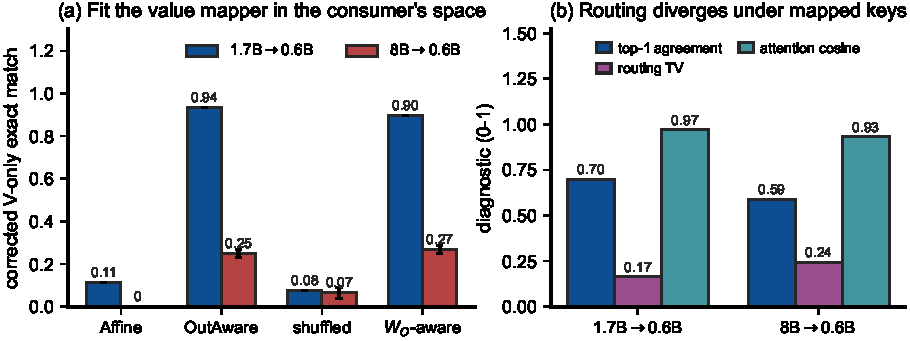
\includegraphics[width=\textwidth]{figures/fig_mappers.pdf}
\caption{(a) Corrected V-only EM by mapper objective. Fitting the mapper in the
consumer's space recovers most of the value arm on the equal-depth pair and about
a quarter on the flagship pair; the shuffled-target control stays near the floor.
(b) Routing diagnostics for the same pairs: attention cosine is high while top-1
agreement is markedly lower and routing total-variation is larger on the
large-gap pair. Top-1 agreement varies over seeds within $0.698$--$0.701$
($1.7$B) and $0.577$--$0.590$ ($8$B).}
\label{fig:mappers}
\end{figure}
\subsection{A consumption adapter recovers transfer}
\label{sec:adapter-results}
We now adapt the consumer instead of the state (Table~\ref{tab:adapter},
Figure~\ref{fig:adapter}). A rank-8 correction of the student's output
projections, trained on calibration teacher KV, raises K/V/Joint EM from
$0.030/0.113/0.000$ to $0.940/0.940/0.827$ for $1.7$B$\to0.6$B and from
$0.000/0.000/0.000$ to $0.792 \pm 0.162/0.357 \pm 0.047/0.470 \pm 0.119$ for
$8$B$\to0.6$B. On the equal-depth pair this nearly reaches the Self reference
($0.899$ unadapted); on the flagship pair it recovers roughly half of Self on the
joint arm and most of the K arm.

The reference frame matters here. The adapter changes the student, so the
appropriate ceiling is the \emph{adapted} Self arm, which the archived summaries
now retain: $0.940 \pm 0.041$ on both pairs. Read against it, the equal-depth
recovery is essentially complete on the K and V arms ($0.940$) and short on the
joint arm ($0.827$), while the flagship recovery is partial on all three
($0.792$, $0.357$, $0.470$). The adapter also raises the student's own readout:
the adapted Self is $0.940 \pm 0.041$ on both pairs, $+0.041$ above the
unadapted $0.899$. Using the unadapted value as the ceiling would therefore
understate the remaining gap on the flagship pair, and on the equal-depth pair
it would credit the recovered K and V arms with a $0.041$ gain over Self that
belongs to the adapter rather than to the transfer.

Both controls fall short of the teacher-KV adapter, which is the evidence that
matters for interpretation. Training the same adapter on the student's own states
yields $0.202/0.345/0.179$ ($1.7$B) and $0.113/0.107/0.119$ ($8$B): the adapter
must see the teacher-state distribution. Training on shuffled-document teacher
states is intermediate, at $0.560/0.345/0.458$ ($1.7$B) and
$0.369/0.113/0.131$ ($8$B). We therefore read the recovery as partly
content-specific and partly an adaptation to teacher-like state distributions in
general; on the $1.7$B joint arm the shuffled control reaches $0.458$ against
$0.827$ for the content-matched adapter. The joint-trained condition also varies
across seeds ($1.7$B joint $0.55$--$0.96$), which the standard deviations in the
table show.

We also ablate which projection carries the correction, on $1.7$B$\to0.6$B
(Table~\ref{tab:ablation}). Adapting the attention output and adapting the value
projection are equally effective at seed 0 (joint arm $0.964$ for both), so this
ablation does not single out \texttt{o\_proj}: any projection on the value path
serves. What the ablation does separate is the addressing path. Adapting
\texttt{q\_proj},\texttt{k\_proj} reaches only $0.625$ on the joint arm, and it
degrades the student's own readout to $0.786$ (from $0.911$) while the
output-side corrections raise it to $0.964$. The content-specificity control
points the same way: an adapter trained on student KV instead of teacher KV
collapses to $0.036$ when \texttt{o\_proj} is adapted and to $0.000$ when
\texttt{v\_proj} is, but stays at $0.411$ when
\texttt{q\_proj},\texttt{k\_proj} are adapted, so much of what the addressing
path learns is generic state adaptation rather than content. The ablation is
seed 0 only except for \texttt{o\_proj}, so we read it as suggestive. Taken with
the mapper results above, it is consistent with the bottleneck sitting on the
value-consumption path rather than on the projections that produce $K$.

Holding a trained adapter fixed and destroying the injected content is the causal
test (Table~\ref{tab:causal}), and we run it on the same $20$-epoch adapter that
Table~\ref{tab:adapter} reports, over three seeds. On $1.7$B$\to0.6$B, correct
teacher KV answers $0.905\pm0.083$ of questions while wrong-document teacher KV,
moment-matched random KV, and an all-zero cache answer at most $0.179$; the
per-seed margins are $+0.714$, $+0.643$, and $+0.857$, and their
document-clustered intervals exclude zero in every seed. The adapter is reading
the injected teacher state rather than solving the task. On $8$B$\to0.6$B the
same test is much weaker: correct KV answers $0.321\pm0.129$ against
$0.107$--$0.286$ for the destroyed arms, the per-seed margins are $+0.107$,
$+0.071$, and $+0.036$, and the mean margin $+0.071$ falls below the $0.10$ our
pre-registered gate requires, with one seed's clustered interval including zero.
We therefore report the flagship causality as unresolved rather than lowering the
bar. One caveat belongs beside that number: repeating the $8$B adapter training
at a fixed seed gave $0.679$ and $0.429$ on the correct arm in two runs, so the
flagship margin is comparable to the training variance of the adapter itself and
the three-seed spread should not be read as a precise estimate.

The repair is also tied to the task distribution, and the tie is tighter than a
cross-domain result alone would suggest (Table~\ref{tab:squadrepair}). Applying
the synthetic-trained mapper and the synthetic-trained adapter to SQuAD without
retraining leaves K-only, V-only, and joint EM at $0.000$ and $0.033$
respectively. The consumption-space mapper makes the SQuAD value arm's
likelihood \emph{worse} ($\dll$ $+4.62$ at seed 0, against $+1.05$ for the
default protocol at the same seed) while EM stays at $0.000$, so on this set it
moves the state further from usable rather than closer. Retraining both
\emph{inside} SQuAD does not recover them either: with fifteen SQuAD calibration
documents and fifteen held-out documents, over three document splits, every
transfer arm---K-only, V-only under each mapper objective, and joint---answers
$0.000$ of the held-out questions, against a held-out Self of $0.333$, $0.200$,
and $0.400$. The adapter is not inert: it raises the student's own SQuAD score to
$0.667$, $0.400$, and $0.400$ on those splits, and to $0.600$ when trained on the
synthetic domain alone. What it raises is the student's reading of \emph{its own}
state; it never makes the transferred state answer SQuAD questions, in domain or
out of it. Two caveats keep this honest: SQuAD supplies only fifteen calibration
documents, far fewer than the synthetic runs use, and the held-out Self ceiling is
$0.20$--$0.40$, which bounds how much either fix could demonstrate. We therefore
read this as consumer compatibility being bound to the task distribution, not as
a claim that no mapper could ever work on SQuAD, and we name the phenomenon
\emph{task-conditioned functional compatibility}: the same producer--consumer
pair is repairable on one distribution and not on another. These runs bound the
claim in two ways. It rests on a single second domain, and a difference in
calibration volume between the two domains is not excluded by them, since the
SQuAD fit sees fifteen documents against the synthetic run's seventy.

\begin{table}[t]
\centering
\small
\caption{Causality test for the consumption adapter: the state changes, the
adapter does not. The adapter is trained on teacher KV (rank 8, $20$ epochs, the
same schedule as Table~\ref{tab:adapter}), frozen, and injected with four
different states; corrected EM, mean $\pm$ std over three seeds. A causal adapter
answers only from the correct teacher state. The $8$B block shows that this test
has little power there: its correct-KV margin ($+0.071$) sits below the
pre-registered $0.10$ threshold and one seed's document-clustered interval
includes zero, so we report it as unresolved. ``Self'' is the student's own cache
under the same adapted model.}
\label{tab:causal}
\begin{tabular}{lcc}
\toprule
Injected state & $1.7$B$\to0.6$B & $8$B$\to0.6$B \\
\midrule
Correct teacher KV (joint)        & $\mathbf{0.905{\pm}0.083}$ & $\mathbf{0.321{\pm}0.129}$ \\
Wrong-document teacher KV          & $0.131{\pm}0.021$ & $0.131{\pm}0.041$ \\
Moment-matched random KV           & $0.095{\pm}0.055$ & $0.125{\pm}0.018$ \\
Zero KV                            & $0.107{\pm}0.071$ & $0.214{\pm}0.095$ \\
\midrule
Self (own cache, adapted)          & $0.952{\pm}0.054$ & $0.929{\pm}0.095$ \\
\bottomrule
\end{tabular}
\end{table}

\begin{table}[t]
\centering
\small
\caption{Projection ablation on $1.7$B$\to0.6$B, seed 0, rank 8, $20$ epochs.
Each condition trains its own adapter from scratch and is then evaluated on all
four arms. Only \texttt{o\_proj} with teacher-KV training was repeated across
seeds (Table~\ref{tab:adapter}, joint arm $0.554$--$0.964$), so the other rows are
single-seed.}
\label{tab:ablation}
\begin{tabular}{llcccc}
\toprule
Adapted projection & Adapter trained on & Self & K-only & V-only & Joint \\
\midrule
\texttt{o\_proj} & teacher KV & $0.964$ & $\mathbf{0.964}$ & $\mathbf{0.964}$ & $\mathbf{0.964}$ \\
\texttt{v\_proj} & teacher KV & $0.964$ & $0.964$ & $0.964$ & $0.964$ \\
\texttt{q\_proj},\texttt{k\_proj} & teacher KV & $0.786$ & $0.821$ & $0.857$ & $0.625$ \\
\midrule
\texttt{o\_proj} & student KV & $0.893$ & $0.036$ & $0.036$ & $0.036$ \\
\texttt{v\_proj} & student KV & $0.857$ & $0.000$ & $0.571$ & $0.000$ \\
\texttt{q\_proj},\texttt{k\_proj} & student KV & $0.536$ & $0.411$ & $0.446$ & $0.411$ \\
\bottomrule
\end{tabular}
\end{table}

\begin{table}[t]
\centering
\small
\caption{Repair on SQuAD, out of domain and within domain. The first block
applies the mapper and adapter fit on the synthetic distribution without
retraining ($n=30$, seed 0). The second block refits both on fifteen SQuAD
calibration documents and evaluates on fifteen held-out documents, over three
document splits, reported as three values. In the within-domain block ``Own
cache'' is the reference under the same fitted condition---unadapted Self for the
mapper row and adapted Self for the adapter row, as in Table~\ref{tab:adapter}.
Every transfer arm is $0.000$ in both blocks.}
\label{tab:squadrepair}
\begin{tabular}{lcccc}
\toprule
Condition & Own cache & K-only & V-only & Joint \\
\midrule
\multicolumn{5}{l}{\emph{Cross-domain: fit on synthetic, evaluated on SQuAD}}\\
Default protocol              & $0.367$ & $0.000$ & $0.000$ & $0.000$ \\
Consumption-space mapper      & $0.367$ & $0.000$ & $0.000$ & $0.000$ \\
Synthetic-trained adapter     & $0.600$ & $0.000$ & $0.033$ & $0.000$ \\
\midrule
\multicolumn{5}{l}{\emph{Within-domain: refit on SQuAD calibration (3 splits)}}\\
Mapper retrained on SQuAD      & $0.33/0.20/0.40$ & $0.000$ & $0.000$ & $0.000$ \\
Adapter retrained on SQuAD     & $0.67/0.40/0.40$ & $0.000$ & $0.000$ & $0.000$ \\
\bottomrule
\end{tabular}
\end{table}

\begin{table}[t]
\centering
\small
\caption{Consumption adapter (rank 8 on \texttt{o\_proj} unless noted),
corrected EM on held-out test, mean $\pm$ std over three seeds. ``Self'' is the
student's own cache under the adapted model, so the reference frame is the
adapted, not the unadapted, student.}
\label{tab:adapter}
\begin{tabular}{llcccc}
\toprule
Pair & Adapter trained on & Self & K-only & V-only & Joint \\
\midrule
\multirow{4}{*}{$1.7$B$\to0.6$B}
 & none            & $0.899{\pm}0.010$ & $0.030{\pm}0.010$ & $0.113{\pm}0.052$ & $0.000$ \\
 & teacher KV      & $0.940{\pm}0.041$ & $\mathbf{0.940{\pm}0.041}$ & $\mathbf{0.940{\pm}0.041}$ & $\mathbf{0.827{\pm}0.237}$ \\
 & student KV      & $0.899{\pm}0.045$ & $0.202{\pm}0.203$ & $0.345{\pm}0.536$ & $0.179{\pm}0.247$ \\
 & shuffled teacher KV & $0.482{\pm}0.064$ & $0.560{\pm}0.021$ & $0.345{\pm}0.055$ & $0.458{\pm}0.152$ \\
\midrule
\multirow{4}{*}{$8$B$\to0.6$B}
 & none            & $0.899{\pm}0.010$ & $0.000$ & $0.000$ & $0.000$ \\
 & teacher KV      & $0.940{\pm}0.041$ & $\mathbf{0.792{\pm}0.162}$ & $\mathbf{0.357{\pm}0.047}$ & $\mathbf{0.470{\pm}0.119}$ \\
 & student KV      & $0.976{\pm}0.021$ & $0.113{\pm}0.010$ & $0.107$ & $0.119{\pm}0.021$ \\
 & shuffled teacher KV & $0.411{\pm}0.099$ & $0.369{\pm}0.109$ & $0.113{\pm}0.052$ & $0.131{\pm}0.021$ \\
\bottomrule
\end{tabular}
\end{table}

\begin{figure}[t]
\centering
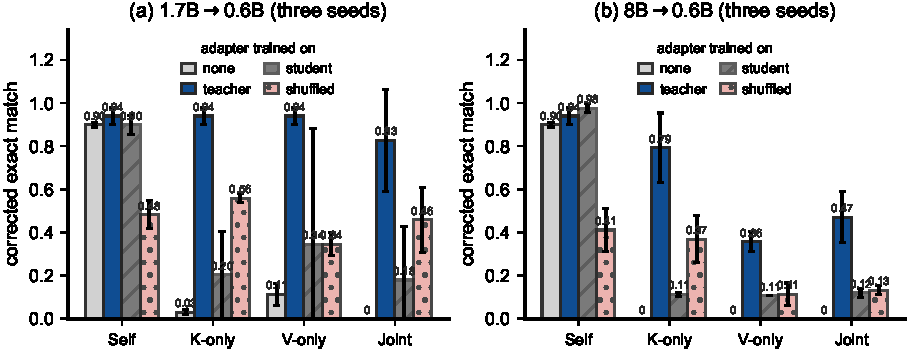
\includegraphics[width=\textwidth]{figures/fig_adapter.pdf}
\caption{Consumption adapter, corrected EM on held-out test (three seeds). A
rank-8 correction of \texttt{o\_proj} trained on calibration teacher KV recovers
the teacher arms; the same adapter trained on student KV does not, and one
trained on shuffled-document teacher KV is intermediate. The ``none'' group is
the unadapted model and ``Self'' is its own cache, which the adapter also moves,
so the adapted Self bars are the reference frame. Error bars are std over seeds
where reported.}
\label{fig:adapter}
\end{figure}

\subsection{Held-out layer selection}
\label{sec:layers-heldout}
A validation scan over all $28$ student layers selects the pair $(12, 16)$ in
every seed, with $L_{12}$ ranked first in all three seeds, so the previously
reported value hotspot is not an artifact of selecting on test
(Figure~\ref{fig:layers}b). Under the corrected metric the selected pair reaches
test EM $0.351$ ($0.339$, $0.357$, $0.357$ across seeds), the post-hoc $(8, 12)$
pair reaches $0.220$, injecting all layers reaches $0.000$, and Self is $0.899$.
A second value pair chosen post hoc for a higher validation score, $(12, 20)$,
reaches only $0.131$, below the validation-selected pair in every seed: selecting
on validation did not cost us anything, and the pre-registered selection is the
stronger one. Selective value injection therefore carries some answer content,
but far too little to constitute task transfer.

\begin{figure}[t]
\centering
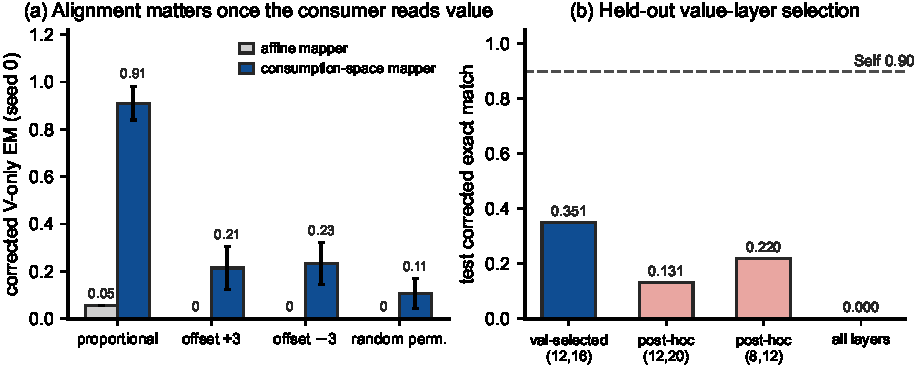
\includegraphics[width=\textwidth]{figures/fig_layers.pdf}
\caption{(a) Layer-map ablation on the equal-depth pair $1.7$B$\to0.6$B (seed 0),
run twice: once with a mapper fit in representation space (affine), where the
value arm is pinned at the floor and the layer map looks irrelevant, and once with
the consumption-space mapper, where the proportional map reaches $0.911$ and the
same scrambling costs most of it. Alignment is invisible until the consumer reads
the state. (b) Held-out value-layer selection on $8$B$\to0.6$B (three seeds): the
validation-selected pair, a post-hoc pair, and all-layer injection, against the
Self reference.}
\label{fig:layers}
\end{figure}
% ============================================================================
\section{Discussion}

\subsection{What the diagnosis does and does not establish}
\label{sec:discussion-scope}
The evidence supports four statements, and we keep them separate rather than
folding them into a single claim about compatibility.
\emph{(i) Evaluation.} Teacher-forced likelihood does not establish functional
cache reuse: content-free caches (wrong document, moment-matched random,
all-zero) reproduce $89$--$105\%$ of the K-only likelihood gain while answering
no question, and the two defects we identify in the implementation we used
earlier inflated greedy EM in our own measurements. The first point holds
independently of any implementation detail; the second covers the code we
audited.
\emph{(ii) Value transfer.} Alignment in raw representation space is
insufficient. The affine mapper minimises representation error and leaves the
value arm unusable, while a mapper fit where the student consumes value recovers
it (Table~\ref{tab:mappers}); with documents as the resampling unit the recovered
arm's clustered CI95 is $[0.839, 0.982]$ against $[0.018, 0.107]$ for the affine
mapper at seed 0, and the two intervals stay disjoint in all three seeds. The
error budget of Table~\ref{tab:errorbudget} makes the distinction quantitative:
raw representation error is smallest for the affine mapper and does not rank the
variants (rank correlation $-0.10$ with EM), while error measured after the
student's attention output and after its $o$-projection does ($-1.00$ and
$-0.80$). Those correlations are computed on the pooled means over five variants
and six runs; the per-run ranges are $[-0.60,-0.10]$, $[-1.00,-0.80]$ and
$[-1.00,-0.80]$, so the ordering holds in every run even though five variants
cannot support a $p$-value.
\emph{(iii) Key transfer.} Mapped teacher keys can perturb the receiver's
routing (top-1 agreement $0.59$--$0.70$ against attention cosine
$0.93$--$0.97$). This is a diagnostic for the key side; the value arm never sees
a mapped key and is not explained by it.
\emph{(iv) Joint handoff.} A full handoff must satisfy both forms of
compatibility and is therefore consistently fragile; it does not reliably combine
the gains of the two components. The joint arm is the lowest of the three teacher
arms on four pairs, is at or above a single arm on the remaining two, and after
adaptation it falls below V-only on the flagship pair.

The role of layer alignment depends on which side is in play, and our own earlier
reading of it was wrong. In representation space the value arm sits at the floor
and scrambling the layer map costs nothing, which we took to mean alignment does
not matter (Section~\ref{sec:layer-align}). In consumption space, where the mapper places value
where the student reads it, the same scrambling collapses V-only EM from $0.911$
to $0.11$--$0.23$. Alignment is a precondition that the ordinary affine mapper
hides behind its own floor, not a quantity the consumer can ignore.

Our evidence does not establish that the recovered information is the teacher's
document content in full. The shuffled-document adapter control is intermediate,
not at the floor, so part of the recovery is an adaptation to teacher-like state
distributions rather than to the specific document. Nor do we identify the
mechanism that makes a state readable: routing divergence is a diagnostic for the
key side, and we measure it rather than intervening on it.

\subsection{Implications}
\label{sec:implications}
If cross-model cache reuse is gated by consumer compatibility rather than by the
existence of a linear map, then evaluations should report task metrics under a
corrected evaluator and include content-free controls, and systems that reuse
caches across models should budget a small consumer-side adaptation. Under our
conditions that adaptation is roughly $0.7$M parameters, trained on calibration
data only, and it recovers most of the K, V, and joint arms on the equal-depth
pair and part of them on the flagship pair. Because that adaptation is fit and
evaluated within one task distribution, we state the requirement as
\emph{task-conditioned functional compatibility}: what has to be compatible is
the producer, the consumer, and the distribution the state was produced on,
taken together.

\subsection{Limitations}
\label{sec:limitations}
\begin{itemize}
\item \textbf{Scope.} All experiments are within one model family (Qwen3,
  $0.6$B--$8$B) and one architecture, with the sizes and head configuration given
  in Section~\ref{sec:models}. We cannot claim cross-family or cross-architecture generality,
  and we did not test teachers outside this family.
\item \textbf{Task distribution.} The adapter is trained on the same task
  distribution it is evaluated on (held-out questions and documents, but the same
  corpus and template). It measures repairability of consumption, not task
  generalization, and the second domain sharpens this: with the mapper and the
  adapter refit \emph{inside} SQuAD, every transfer arm still answers $0.000$ of
  the held-out questions across three document splits
  (Table~\ref{tab:squadrepair}). SQuAD supplies only fifteen calibration
  documents and its held-out Self is $0.20$--$0.40$, so we read this as
  compatibility being bound to the task distribution rather than as proof that no
  mapper can work there, and we call it \emph{task-conditioned}. The alternative
  reading---that the second domain fails only because it supplies far less
  calibration data---is not excluded by these runs and is the first thing a
  follow-up should separate.
\item \textbf{Corpus effects.} Every document shares a template, and each
  document is reused across about seven questions (test: $56$ questions from $8$
  documents). Wrong-document controls are therefore conservative as content
  controls, since two documents differ mainly in the entities they mention. The
  four-arm EM table reports std over seeds and no interval, but document-clustered
  EM intervals (eight clusters per seed) are computed for all three seeds from the
  archived per-sample rows and are quoted in Section~\ref{sec:teacher-states}. They are wider than
  per-sample intervals and they confirm the ordering rather than overturning
  it---on $8$B$\to4$B, V-only is $0.43$--$0.45$ with intervals excluding zero,
  against a Self of $0.80$--$0.84$. The std over seeds remains too narrow to lean
  on, and the clustered intervals still leave that pair's V-only arm far below
  Self.
\item \textbf{Variance.} The $1.7$B adapter's joint arm ranges from $0.55$ to
  $0.96$ across seeds, and several likelihood quantities have large seed-to-seed
  spread (for example $8$B$\to1.7$B K-only $+1.04 \pm 1.53$). Three seeds is a
  small sample; we report std rather than intervals for most arms.
\item \textbf{Mapper family.} We test linear and ridge mappers, including
  consumer-space variants. Nonlinear mappers, and mappers trained on more
  calibration data, remain untested; a stronger mapper could change how much of
  the failure is attributable to consumption rather than to mapping.
\item \textbf{Evaluator provenance.} Our corrected numbers come from our own
  evaluator, validated against a full-prefill reference on the complete $56$-item
  Self test set of three student sizes (Figure~\ref{fig:evalcheck}) and again on
  the $30$-item SQuAD Self set. The agreement is on the extracted answer
  (normalized-EM $0.929$--$0.982$) and on the first-token distribution (top-1
  agreement $0.929$--$0.982$, median $KL$ $0.001$--$0.005$ nats), not
  token-for-token: greedy tokenization diverges on $7$--$21\%$ of items depending
  on student size, and the largest single logit error is $1.344$. We attribute
  that residual rather than leaving it unexplained---repeated capture, the cache
  round-trip, and explicit position offsets are all exact, and the entire
  difference belongs to the attention kernel path, a numerical difference at
  bf16 precision rather than an implementation defect. Legacy numbers are
  reported for comparison in the supplementary material rather than in the main
  text.
\item \textbf{Unexplained baseline spread.} Self EM differs by student
  ($0.899$ for the three $0.6$B students, $0.440$ for the two $1.7$B students,
  $0.815$ for the $4$B student). Raw and normalized exact match agree for every
  student ($0.911$, $0.429$, $0.804$ raw against $0.911$, $0.429$, $0.804$
  normalized; $0$ items flip from wrong to right under normalization) and the
  failure counts are $5$, $32$, and $11$ of $56$. Classifying the archived
  generations, every $1.7$B failure is a well-formed answer naming the wrong
  entity or value---another component or plant of the same template, or the
  opposite polarity on the yes/no questions---with no refusal, no repetition
  loop, no empty output and no generation truncated at the decode cap; the
  $0.6$B and $4$B failures are of the same kind. The $1.7$B dip is therefore
  task error, not a formatting or extraction artifact, but we still cannot
  explain why that size is the weakest. It does not affect within-pair arm
  comparisons, which is what our claims rest on, but it means absolute EM
  levels are not comparable across pairs.
\item \textbf{Partial seed coverage.} Two results remain seed 0 only: the
  repaired-regime layer scrambling (Section~\ref{sec:layer-align}) and the projection ablation of
  Table~\ref{tab:ablation}. The adapter causality test, the mapper comparisons,
  the second domain, and both control suites were run for all three seeds, as
  were all four-arm scans. Where a comparison matters for a headline claim we
  used a three-seed run.
\item \textbf{Flagship causality.} With the final $20$-epoch adapter frozen,
  destroying the injected content separates the correct arm from the
  controls clearly on $1.7$B$\to0.6$B ($0.905\pm0.083$ against at most $0.179$,
  margins $+0.71$ to $+0.86$ with clustered intervals excluding zero) but not on
  $8$B$\to0.6$B ($0.321\pm0.129$ against $0.107$--$0.286$, mean margin $+0.071$,
  one clustered interval containing zero). We cannot rule out that part of the
  flagship recovery is generic adaptation to teacher-like states.
\item \textbf{Adapter training variance.} Repeating the flagship adapter
  training at a fixed seed gave $0.679$ and $0.429$ on the correct causal arm in
  two runs. The $8$B margin ($+0.071$) is therefore comparable to the training
  variance of the adapter itself, which is a second reason not to read the
  flagship causality as established. We report three-seed means and do not treat
  the seed spread as a confidence statement.
\item \textbf{Withdrawn claims.} The pre-registered G0 gate and all previously
  published EM figures for this project are withdrawn (Section~\ref{sec:analyses}). The
  likelihood results survive, but they are likelihood results.
\end{itemize}

\subsection{Future work}
\label{sec:future-work}
Three directions follow: (i) a routing-aware key mapper that optimizes the
attention logits rather than the key vectors, to test whether the residual gap on
large-gap pairs is closable; (ii) cross-family evaluation (for example
Qwen$\to$Llama) to test the boundary of the consumption adapter; and (iii)
systems measurements of mapper and adapter latency against re-prefilling, which
should replace the parameter-count heuristic of Appendix~\ref{app:cost} with
measured cost.

\subsection{Conclusion}
\label{sec:conclusion}
Cross-model KV transfer is a state--consumer compatibility problem with two sides
that our four-arm design keeps apart. Mapped teacher keys perturb the receiver's
routing (the key side), while mapped values stay unusable until the mapper is fit
where the receiver consumes them, however small their raw representation error is
(the value side). Standard linear maps make teacher state predictable and raise
teacher-forced likelihood, but under a corrected evaluator those states do not
answer questions, and content-free caches reproduce the likelihood gains that
made the transfer look real. Mappers fit in the consumer's space recover the value
arm on the equal-depth pair without touching a single consumer weight---which the
error budget confirms is the right target, since raw representation error does not
rank the mappers by task performance while error measured where the receiver reads
the state does---and a small rank-8 adaptation of the student's output projections
recovers most of the K, V, and joint arms there. On the flagship pair the frozen
adapter reads the injected content on the equal-depth pair but not on the
flagship one, where the margin stays inside our pre-registered noise band, and on
a second domain neither the mapper nor the adapter repairs anything even when
both are refit inside that domain. Layer alignment returns to the picture once the
consumer reads the state, which the ordinary affine mapper hides. Evaluation of
cross-model cache reuse should measure task performance with content controls,
and reuse systems should expect to adapt the consumer within the task
distribution where the adaptation is fit.

% ============================================================================
\section{Reproducibility statement}
\begin{sloppypar}
Data generation, model loading, the corrected evaluator, the control suite, the
consumer-space mappers, and the consumption adapter are implemented in
\texttt{experiments/phaseB\_*.py}; the analysis scripts that recompute the
document-clustered statistics and classify the baseline failures are in
\texttt{scripts/}. Figures are generated by
\texttt{paper/figures/gen\_paper\_figures.py}, which records the transcribed
values and their provenance. Corrected four-arm scans, controls, alignment
ablations, held-out layer selection, mapper comparisons, adapter runs, and the
per-sample decomposition write JSON reports under \texttt{reports/}
(\texttt{phaseB\_fourarm\_seed*.json},
\texttt{phaseB\_controls\_*.json},
\texttt{phaseB\_mechanism\_*.json},
\texttt{phaseB\_outaware\_*.json},
\texttt{phaseB\_adapter\_*.json},
\texttt{phaseB\_alignment\_repaired\_*.json},
\texttt{phaseB\_evalcheck\_seed0.json},
\texttt{phaseB\_selfdiag\_seed0.json},
\texttt{phaseB\_squad\_seed*.json},
\texttt{phaseB\_squad\_outaware\_seed0.json},
\texttt{phaseB\_squad\_adapter\_seed0.json}, and
\texttt{factorial\_analysis.json} for the decomposition,
\texttt{phaseB\_evalcheck\_residual\_seed0.json},
\texttt{phaseB\_evalcheck\_attrib.json} and
\texttt{phaseB\_evalcheck\_squad.json} for the evaluator attribution,
\texttt{phaseB\_adapter\_causal20\_*.json} for the frozen
adapter causality test, \texttt{phaseB\_squadwithin\_split*.json} for the
within-domain SQuAD repair, \texttt{phaseB\_errorbudget\_*.json} for the error
budget, and \texttt{cluster\_stats\_audit3.json} for the document-clustered
intervals; the superseded cost figure replaced in Appendix~\ref{app:cost} is
archived under \texttt{reports/archive/}). A
detailed correction note (\texttt{paper/audit/METRIC\_CORRECTION.md}) documents
the evaluator defects, the legacy numbers they produced, and the mapping from
each revised claim to its report.
\end{sloppypar}
\begin{thebibliography}{10}

\bibitem{bansal2021stitching}
Yamini Bansal, Preetum Nakkiran, and Boaz Barak.
\newblock Revisiting model stitching to compare neural representations.
\newblock In {\em Advances in Neural Information Processing Systems}, 2021.

\bibitem{chen2023accelerating}
Charlie Chen, Sebastian Borgeaud, Geoffrey Irving, et~al.
\newblock Accelerating large language model decoding with speculative sampling.
\newblock {\em arXiv preprint arXiv:2302.01318}, 2023.

\bibitem{dao2022flashattention}
Tri Dao, Dan Fu, Stefano Ermon, Atri Rudra, and Christopher R{\'e}.
\newblock Flashattention: Fast and memory-efficient exact attention with
  io-awareness.
\newblock {\em Advances in Neural Information Processing Systems}, 35, 2022.

\bibitem{dery2026latentalign}
Lucio~M. Dery, Zohar Yahav, Henry Prior, Qixuan Feng, Jiajun Shen, and Arthur
  Szlam.
\newblock Latent space communication via k-v cache alignment.
\newblock {\em arXiv preprint arXiv:2601.06123}, 2026.

\bibitem{dettmers2024qlora}
Tim Dettmers, Artidoro Pagnoni, Ari Holtzman, and Luke Zettlemoyer.
\newblock Qlora: Efficient finetuning of quantized language models.
\newblock {\em Advances in Neural Information Processing Systems}, 36, 2024.

\bibitem{frantar2023gptq}
Elias Frantar, Saleh Ashkboos, Torsten Hoefler, and Dan Alistarh.
\newblock Gptq: Accurate post-training quantization for generative pre-trained
  transformers.
\newblock {\em arXiv preprint arXiv:2210.17323}, 2023.

\bibitem{fu2026c2c}
Tianyu Fu, Zihan Min, Hanling Zhang, Jichao Yan, Guohao Dai, Wanli Ouyang, and
  Yu~Wang.
\newblock Cache-to-cache: Direct semantic communication between large language
  models.
\newblock In {\em International Conference on Learning Representations}, 2026.
\newblock arXiv:2510.03215.

\bibitem{heo2026crossmodel}
Taekyung Heo, Rasoul Shafipour, Ritchie Zhao, Maximilian Golub, Mohammad~Mahdi
  Kamani, Ritika Borkar, Makesh~Tarun Chandran, Pantea Zardoshti, and
  Bita~Darvish Rouhani.
\newblock Cross-model kv cache transfer in llm families: A closed-form linear
  mapping for prefill reuse.
\newblock {\em arXiv preprint arXiv:2608.03893}, 2026.

\bibitem{hinton2015distilling}
Geoffrey Hinton, Oriol Vinyals, and Jeff Dean.
\newblock Distilling the knowledge in a neural network.
\newblock {\em arXiv preprint arXiv:1503.02531}, 2015.

\bibitem{lee2026translators}
Jin-woo Lee, Minkyung Song, Junghyun Oh, Seunghoon Han, Soyoung Park, Gwangseon
  Jang, and Sungsu Lim.
\newblock Mixture-of-translators: Translating kv caches across heterogeneous
  large language models.
\newblock {\em arXiv preprint arXiv:2607.28979}, 2026.

\bibitem{leviathan2023fast}
Yan Leviathan, Matan Kalman, and Yossi Matias.
\newblock Fast inference from transformers via speculative decoding.
\newblock {\em International Conference on Machine Learning}, pages
  19274--19290, 2023.

\bibitem{su2024rope}
Jianlin Su, Murtadha Ahmed, Yu~Lu, Shengfeng Pan, Wen Bo, and Yunfeng Liu.
\newblock Roformer: Enhanced transformer with rotary position embedding.
\newblock {\em Neurocomputing}, 568:127063, 2024.

\bibitem{dare2024icml}
Le Yu, Bowen Yu, Haiyang Yu, Fei Huang, and Yongbin Li.
\newblock Language models are super mario: Absorbing abilities from homologous
  models as a free lunch.
\newblock {\em International Conference on Machine Learning}, 2024.
\newblock arXiv:2311.03099.

\bibitem{kivi2024icml}
Zirui Liu, Jiayi Yuan, Hongye Jin, Shaozhuo Zhai, Yuanzhi Chen, et~al.
\newblock Kivi: A tuning-free asymmetric 2bit quantization for kv cache.
\newblock {\em International Conference on Machine Learning}, 2024.
\newblock arXiv:2402.02750.

\bibitem{kvquant2024nips}
Coleman Hooper, Sehoon Kim, Hiva Mohammadzadeh, Michael~W. Mahoney,
  Kurt Keutzer, and Amir Gholami.
\newblock Kvquant: Towards 10 million context length llm inference with
  kv cache quantization.
\newblock {\em Advances in Neural Information Processing Systems}, 37, 2024.
\newblock arXiv:2401.18079.

\bibitem{ties2023merging}
Prateek Yadav, Derek Tam, Leshem Choshen, Colin Raffel, and Mohit Bansal.
\newblock Ties-merging: Resolving interference when merging models.
\newblock {\em Advances in Neural Information Processing Systems}, 36, 2023.
\newblock arXiv:2306.01708.

\bibitem{touvron2023llama}
Hugo Touvron, Thibaut Lavril, Gautier Izacard, et~al.
\newblock Llama: Open and efficient foundation language models.
\newblock {\em arXiv preprint arXiv:2302.13971}, 2023.

\bibitem{vaswani2017attention}
Ashish Vaswani, Noam Shazeer, Niki Parmar, et~al.
\newblock Attention is all you need.
\newblock {\em Advances in Neural Information Processing Systems}, 30, 2017.

\end{thebibliography}

\appendix

\section{Decomposition of the likelihood deltas}
\label{app:factorial}
This appendix holds the exploratory likelihood decomposition that
Section~\ref{sec:layer-align} refers to; it is moved out of the main text
because a likelihood gain is not by itself evidence of functional transfer
(Section~\ref{sec:controls}). Because corrected EM of every teacher arm is at the
floor, the four-arm design can only be decomposed on the likelihood scale.
Table~\ref{tab:factorial} reports the K main effect (K-only $-$ Self), the V main
effect (V-only $-$ Self), and their interaction
(Joint $-$ K-only $-$ V-only $+$ Self), computed per sample and averaged over
seeds from the same runs as Table~\ref{tab:main}.

Several patterns follow, and we label them exploratory. The V main effect is
positive on four pairs and negative on two, with the largest positive value on
$8$B$\to1.7$B ($+5.63 \pm 0.04$) and the largest negative on $4$B$\to0.6$B
($-1.22 \pm 0.05$). The interaction is positive for the two large-to-small-$0.6$B
pairs ($+2.12 \pm 0.07$ for $8$B$\to0.6$B and $+2.15 \pm 0.55$ for
$4$B$\to0.6$B) and negative for the other four ($-2.06 \pm 0.22$,
$-2.67 \pm 0.09$, $-1.98 \pm 1.79$, and $-3.50 \pm 0.12$). Its sign therefore
varies by pair; no single K$\times$V interaction story holds across the six
pairs, and all of these are likelihood effects rather than task effects.

For the flagship pair we can test the headline asymmetry directly on per-sample
differences ($n=56$): the paired K-minus-V difference is $+2.457$
(CI95 $[+1.73, +3.29]$, $p=1.4\times10^{-9}$) at seed 0, $+2.720$
($p=1.4\times10^{-10}$) at seed 1, and $+3.361$ ($p=7.5\times10^{-11}$) at seed
2. On this pair the K arm improves likelihood more than the V arm by a clear
margin, in every seed. That is a statement about likelihood; on corrected EM both
arms are $0.000$.

\begin{table}[t]
\centering
\small
\caption{Decomposition of the likelihood deltas (exploratory), three seeds,
$n=56$. K main effect $=$ K-only $-$ Self; V main effect $=$ V-only $-$ Self;
interaction $=$ Joint $-$ K-only $-$ V-only $+$ Self, on per-sample mean answer
log-likelihood. The K and V columns equal the corresponding $\dll$ columns of
Table~\ref{tab:main} and are repeated for reference.}
\label{tab:factorial}
\begin{tabular}{lccc}
\toprule
Pair & K main effect & V main effect & K$\times$V interaction \\
\midrule
$8$B$\to0.6$B   & $+2.62{\pm}0.29$ & $-0.23{\pm}0.19$ & $+2.12{\pm}0.07$ \\
$4$B$\to1.7$B   & $+2.90{\pm}0.09$ & $+2.91{\pm}0.21$ & $-3.50{\pm}0.12$ \\
$4$B$\to0.6$B   & $+1.58{\pm}0.02$ & $-1.22{\pm}0.05$ & $+2.15{\pm}0.55$ \\
$8$B$\to1.7$B   & $+1.04{\pm}1.53$ & $+5.63{\pm}0.04$ & $-1.98{\pm}1.79$ \\
$1.7$B$\to0.6$B & $-0.82{\pm}0.02$ & $+0.63{\pm}0.17$ & $-2.06{\pm}0.22$ \\
$8$B$\to4$B     & $+8.52{\pm}0.28$ & $+2.52{\pm}0.07$ & $-2.67{\pm}0.09$ \\
\bottomrule
\end{tabular}
\end{table}

\section{Cost heuristic for transmitting a mapper instead of a cache}
\label{app:cost}
For completeness: with the mapper actually used in this paper---one affine map
per (layer, head), $L_S\cdot H\cdot(D^2+D)$ parameters per side, both sides
stored in fp32---the parameter count for a $28$-layer student is $7.40$M
($28.2$ MiB) against $112$ KiB per token of fp16 KV, which puts the byte
crossover near $260$ tokens. The number is a heuristic: it counts mapper
parameters rather than transfer time, it ignores quantization and caching, and it
does not bear on the state--consumer findings above. An earlier version of this
text quoted a much larger crossover, because it counted a single
$1024\times1024$ map per layer rather than the per-(layer, head) map defined in
Section~\ref{sec:mappers}.

\end{document}
